\chapter{Modelo de regresión lineal múltiple}

\section{Modelo. Hipétesis del modelo}
Buscamos un modelo que nos permita establecer una relación entre las variables aleatorias $X_1,\ldots,X_k$ e $Y$. El modelo que vamos a estudiar es el siguiente
\begin{align*}
    y_i = \beta_0 + \beta_1 x_{1i} + \ldots + \beta_k x_{ki} + u_i, \ i = 1,\ldots,n,
\end{align*}
donde $x_{ji}$ es el valor de la variable $X_j$ en el $i$-ésimo individuo, $j = 1,\ldots,k$, $i=1,\ldots,n$.

\underline{Hipótesis del modelo}:
\begin{enumerate}
    \item[H1.] $E(u_i) = 0$, $i = 1,\ldots,n$.
    \item[H2.] $Var(u_i) = \sigma^2$, $i = 1,\ldots,n$ (Homocedasticidad).
    \item[H3.] $u_i \sim N(0,\sigma^2)$, $i = 1,\ldots,n$ (Normalidad).
    \item[H4.] $E(u_i - u_j) = 0$, $i,j=1,..,n$, $i \not = j$ (Independencia).
    \item[H5.] $n > k+1$.
    \item[H6.] No existen relaciones lineales entre las variables $X_i$ (Ausencia de multicolinealidad).
\end{enumerate}
Podemos expresar este modelo de forma matricial, si definimos
\begin{align*}
    \vec{y} = \begin{bmatrix}
                  y_1    \\
                  \vdots \\
                  y_n
              \end{bmatrix} \in \mathbb{R}^n, \ \vec{\beta} = \begin{bmatrix}
                                                                  \beta_0 \\
                                                                  \vdots  \\
                                                                  \beta_k
                                                              \end{bmatrix} \in \mathbb{R}^{k+1}, \ \vec{u} = \begin{bmatrix}
                                                                                                                  u_1    \\
                                                                                                                  \vdots \\
                                                                                                                  u_n
                                                                                                              \end{bmatrix} \in \mathbb{R}^n, \\
    X = \begin{bmatrix}
            1      & x_{11} & x_{21} & \cdots & x_{k1} \\
            1      & x_{12} & x_{22} & \cdots & x_{k2} \\
            \vdots & \vdots & \vdots & \ddots & \vdots \\
            1      & x_{1n} & x_{2n} & \cdots & x_{n}
        \end{bmatrix} \in \mathcal{M}_{n \times (k+1)} (\mathbb{R}).
\end{align*}
Entonces, podemos expresar el modelo anterior como
\begin{align*}
    \vec{y} = X \vec{\beta} + \vec{u}
\end{align*}
Las hipótesis H1, H2, H3 y H4, se traducen en $\vec{u} \sim N_n(\vec{0}, \sigma^2 I_n)$, de donde deducimos que $\vec{y} \sim N_n(X\vec{\beta}, \sigma^2 I_n)$. La hipótesis H5 sigue siendo la misma ($n > k+1$). La hipótesis H6 se traduce en que $rg(X) = k+1$.

\underline{Hipótesis del modelo}:
\begin{enumerate}
    \item[H1.] $E(y_i | x_{1i},\ldots,x_{ki}) = \beta_0 + \beta_1 x_{1i} + \ldots + \beta_k x_{ki}$, $i = 1,,,.,n$ (Linealidad).
    \item[H2.] $Var(y_i | x_{1i},\ldots,x_{ki}) = \sigma^2$, $i = 1,\ldots,n$ (Homocedasticidad).
    \item[H3.] $y_i | x_{1i},\ldots,x_{ki} \sim N(\beta_0 + \beta_1 x_{1i} + \ldots + \beta_k x_{ki}, \sigma^2)$, $i = 1,\ldots,n$.
    \item[H4.] $Cov(y_i,y_j) = 0$, $i,j = 1,\ldots,n$, $i \not = j$.
    \item[H5.] $n > k+1$.
    \item[H6.] No existen relaciones lineales entres las variables $X_j$ (Ausencia de multicolinealidad).
\end{enumerate}
La interpretacón de los $\beta_j$ es la siguiente:
\begin{itemize}
    \item $E(y_1 | x_{1i} = \ldots = x_{ki} = 0) = \beta_0$.
    \item $E(y_i | x_{1i}, \ldots., x_{ji} +1, \ldots., x_{ki}) - E(y_i | x_{1i}, \ldots., x_{ji}, \ldots., x_{ki}) = \beta_j$. Para $j=1,\ldots,k$, $\beta_j$ es la variación media de la variable respuesta cuando $x_{ji}$ aumenta en una unidad y el resto de variables permanece constante.
\end{itemize}

\section{Estimación de los parámetros}
Podemos estimar $E(y_i | x_{i1},\ldots,x_{ki})$ con
\begin{align*}
    \widehat{y}_i = \widehat{E(y_i | x_{i1},\ldots,x_{ki})} = \widehat{\beta}_0 + \widehat{\beta}_1 x_{1i} + \ldots + \widehat{\beta}_k x_{ki}
\end{align*}
Apliquemos mínimos cuadrados para ver quienes serían $\widehat{\beta}' = (\widehat{\beta}_0,\ldots,\widehat{\beta}_k)$. Definimos
\begin{align*}
    M(\beta_0,\ldots,\beta_k) = \sum_{i=1}^{n} (y_i - \beta_0 - \beta_1 x_{1i} - \ldots - \beta_k x_{ki})^2.
\end{align*}
Sus derivadas parciales son
\begin{align*}
    \frac{\partial M}{\partial \beta_0} (\beta_0,\ldots,\beta_k) & = -2 \sum_{i=1}^{n} (y_i - \beta_0 - \beta_1 x_{1i} - \ldots - \beta_k x_{ki})                            \\
    \frac{\partial M}{\partial \beta_j} (\beta_0,\ldots,\beta_k) & = -2\sum_{i=1}^{n} x_{ji} (y_i - \beta_0 - \beta_1 x_{1i} - \ldots - \beta_k x_{ki}, \ \ \ j = 1,\ldots,k
\end{align*}
Haciendo algunos cálculos se llega a que se tiene que cumplir:
\begin{align*}
    \sum_{i=1}^{n} (y_i - \beta_0 - \beta_1 x_{x1i} - \ldots - \beta_k x_{ki})        & = 0                       \\
    \sum_{i=1}^{n} x_{ji} (y_i - \beta_0 - \beta_1 x_{x1i} - \ldots - \beta_k x_{ki}) & = 0, \ \ \ j = 1,\ldots,k
\end{align*}
Si denotamos $e_i = y_i - \widehat{y}_i$, $i = 1,\ldots,n$, dichas condiciones se traducen como
\begin{align*}
    \sum_{i=1}^{n} e_i        & = 0                       \\
    \sum_{i=1}^{n} x_{ji} e_i & =0, \ \ \ j = 1,\ldots,k,
\end{align*}
que se conocen como las ecuaciones normales de la regresión. Desarrollando cálculos
\begin{align*}
    \sum_{i=1}^{n} y_i        & = n \widehat{\beta}_0 + \widehat{\beta}_1 \sum_{i=1}^{n} x_{1i} + \widehat{\beta}_2 \sum_{i=1}^{n} x_{2i} + \ldots + \widehat{\beta}_k \sum_{i=1}^{n} x_{ki}                                     \\
    \sum_{i=1}^{n} x_{1i} y_i & = \widehat{\beta}_0 \sum_{i=1}^{n} x_{1i} + \widehat{\beta}_1 \sum_{i=1}^{n} x_{1i}^2 + \widehat{\beta}_2 \sum_{i=1}^{n} x_{1i} x_{2i} + \ldots + \widehat{\beta}_k \sum_{i=1}^{n} x_{1i} x_{ki} \\
    \sum_{i=1}^{n} x_{2i} y_i & = \widehat{\beta}_0 \sum_{i=1}^{n} x_{2i} + \widehat{\beta}_1 \sum_{i=1}^{n} x_{1i} x_{2i} + \widehat{\beta}_2 \sum_{i=1}^{n} x_{2i}^2 + \ldots + \widehat{\beta}_k \sum_{i=1}^{n} x_{2i} x_{ki} \\
                              & \vdots                                                                                                                                                                                           \\
    \sum_{i=1}^{n} x_{ki} y_i & = \widehat{\beta}_0 \sum_{i=1}^{n} x_{ki} + \widehat{\beta}_1 \sum_{i=1}^{n} x_{1i} x_{ki} + \widehat{\beta}_2 \sum_{i=1}^{n} x_{2i} x_{ki} + \ldots + \widehat{\beta}_k \sum_{i=1}^{n} x_{ki}^2
\end{align*}
De manera matricial nos quedaría
\begin{align*}
    X'\vec{y} = X'X\widehat{\vec{\beta}} \Longleftrightarrow \widehat{\vec{\beta}} = (X'X)^{-1}X'\vec{y}.
\end{align*}
Nótese que $(X'X)^{-1}$ existe por H6.

\begin{obs}
    \begin{align*}
        \frac{\sum_{i=1}^{n} e_i^2}{\sigma^2} \sim \chi^2_{n-(k+1)} \equiv \chi^2_{n-k-1}
    \end{align*}
    Entonces
    \begin{align*}
        E\left( \frac{\sum_{i=1}^{n} e_i^2}{\sigma^2}  \right) = n-k-1 \ \ \text{ y } \ \ Var\left( \frac{\sum_{i=1}^{n} e_i^2}{\sigma^2} \right) = 2(n-k-1).
    \end{align*}
    Si definimos
    \begin{align*}
        \boxed{
            s_R^2 = \frac{\sum_{i=1}^{n} e_i^2}{n-k-1}
        }
    \end{align*}
    Tenemos que
    \begin{align*}
        E(s_R^2)   & = \frac{1}{n-k-1}E\left( \sum_{i=1}^{n} e_i^2 \right) = \frac{1}{n-k-1} \sigma^2(n-k-1) = \sigma^2                                    \\
        Var(s_R^2) & = \frac{1}{(n-k-1)^2}Var\left( \sum_{i=1}^{n} e_i^2 \right) = \frac{1}{(n-k-1)^2} 2(n-k-1) (\sigma^2)^2 = \frac{2(\sigma^2)^2}{n-k-1}
    \end{align*}
    Todo esto nos dice que $s_R^2$ es un estimador insesgado para $\sigma^2$.
\end{obs}

\section{Propiedades de los estimadores}
Ya hemos probado que $\widehat{\vec{\beta}} = (X'X)^{-1}X'\vec{y}$ y que $\vec{y} = N_n(X\vec{\beta}, \sigma^2 I_n)$, de donde deducimos que $\widehat{\vec{\beta}} \sim N_{k+1}(\vec{\beta}, \sigma^2 (X'X)^{-1})$. Veámoslo.
\begin{proof}
    \begin{align*}
        E(\widehat{\vec{\beta}})   & = (X'X)^{-1}XE(\vec{y}) = (X'X)^{-1}X\vec{\beta} = \vec{\beta}                                                                                  \\
        Cov(\widehat{\vec{\beta}}) & = (X'X)^{-1}XCov(\vec{y})X(X'X)^{-1} = (X'X)^{-1}X'\sigma I_n X(X'X)^{-1} = \sigma^2 (X'X)^{-1}                                                 \\
                                   & = \begin{bmatrix}
                                           Var(\widehat{\beta}_0)                   & Cov(\widehat{\beta}_0, \widehat{\beta}_1)     & \cdots & Cov(\widehat{\beta}_0, \widehat{\beta}_k) \\
                                           Cov(\widehat{\beta}_0,\widehat{\beta}_1) & Var(\widehat{\beta}_2)                        & \cdots & Cov(\widehat{\beta}_2, \widehat{\beta}_k) \\
                                           \vdots                                   & \vdots                                        & \ddots & \vdots                                    \\
                                           Cov(\widehat{\beta}_0,\widehat{\beta}_k) & Cov(\widehat{\beta}_0, \widehat{\beta}_{k-1}) & \cdots & Var(\widehat{\beta}_k)
                                       \end{bmatrix}
    \end{align*}
    Así, $\widehat{\beta}_j \sim N(\beta_j, \sigma^2{q_{j+1,j+1}})$, siendo $q_{j+1,j+1}$ el elemento $(j+1)$-ésimo de la diagonal de $(X'X)^{-1}$.
\end{proof}

\section{Intervalos de confianza para los parámetros}

\subsection{Intervalos de confianza para $\beta_j$, $j=0,1,\ldots,k$}
Supondremos que $\sigma^2$ es desconocido (que suele ser lo común en la realidad). Sea $j \in \{0,1,\ldots,k\}$, entonces $\widehat{\beta}_j \sim N(\beta_j, \sigma^2{q_{j+1,j+1}})$, tipificando
\begin{align*}
    \frac{\widehat{\beta}_j - \beta_j}{\sigma\sqrt{q_{j+1,j+1}}} \sim N(0,1).
\end{align*}
Sabemos además que
\begin{align*}
    \frac{(n-k-1)s_R^2}{\sigma^2} = \frac{\sum_{i=1}^{n} e_i^2}{\sigma^2} \sim \chi^2_{n-k-1}.
\end{align*}
Entonces
\begin{align*}
    \dfrac{\dfrac{\widehat{\beta}_j - \beta_j}{\sigma\sqrt{q_{j+1,j+1}}}}{\sqrt{\dfrac{(n-k-1)s_R^2}{\sigma^2} \cdot \dfrac{1}{n-k-1}}} = \frac{\widehat{\beta}_j - \beta_j}{s_R\sqrt{q_{j+1,j+1}}} \sim t_{n-k-1}.
\end{align*}
Entonces
\begin{align*}
    IC_{1-\alpha}(\beta_j) = \left( \widehat{\beta}_j - t_{n-k-1, 1 -\alpha/2} \cdot s_R \sqrt{q_{j+1,j+1}}, \widehat{\beta}_j + t_{n-k-1, 1 -\alpha/2} \cdot s_R \sqrt{q_{j+1,j+1}} \right),
\end{align*}
siendo $t_{n-k-1, 1 -\alpha/2}$ el cuantil $1 - \alpha/2$ de la distribución $t_{n-k-1}$.

\subsection{Intervalo de confianza para $\sigma^2$}
Fijamos $\alpha \in (0,1)$. Sean $0 < a < b$, entonces
\begin{align*}
    1 - \alpha = P(a < \sigma^2 < b) & = P\left( \frac{1}{b} < \frac{1}{\sigma^2} < \frac{1}{a}\right)                                  \\
                                     & = P\left( \frac{(n-k-1)s^2_R}{b} < \frac{(n-k-1)s^2_R}{\sigma^2} < \frac{(n-k-1)s^2_R}{a}\right)
\end{align*}
Sabemos que
\begin{align*}
    \frac{(n-k-1)s^2_R}{\sigma^2} = \frac{\sum_{i=1}^{n} e_i^2}{\sigma^2} \sim \chi^2_{n-k-1}.
\end{align*}
Entonces
\begin{align*}
    IC_{1-\alpha}(\sigma^2) = \left( \frac{(n-k-1)s^2_R}{\chi^2_{n-k-1,1-\alpha/2}}, \frac{(n-k-1)s^2_R}{\chi^2_{n-k-1,\alpha/2}} \right),
\end{align*}
siendo $\chi^2_{n-k-1,1-\alpha/2}$ y $\chi^2_{n-k-1,\alpha/2}$ los cuantiles $1-\alpha/2$ y $\alpha/2$ de la distribución $\chi^2_{n-k-1}$ respectivamente.

\section{Contrastes de hipótesis para los coeficientes de regresión}

\subsection{Contrastes de significación individuales}
Queremos saber si la variable $X_j$ es influyente en el modelo. Para cada $j = 1,\ldots,k$ planteamos el contraste
\begin{align*}
    \left\{ \begin{array}{lcc}
                H_0 \ : \ \beta_j = 0      \\
                H_1 \ : \ \beta_j \not = 0 \\
            \end{array}
    \right.
\end{align*}
Este contraste quiere decir si hay suficiente evidencia en la muestra para afirmar que la variable $X_j$ tiene una influencia lineal significativa en el modelo.

Fijemos nivel de signifación $\alpha$.
\begin{enumerate}
    \item[I)] Mediante intervalos de confianza. Sabemos que
          \begin{align*}
              IC_{1-\alpha}(\beta_j) = \left( \widehat{\beta}_j - t_{n-k-1, 1 -\alpha/2} \cdot s_R \sqrt{q_{j+1,j+1}}, \widehat{\beta}_j + t_{n-k-1, 1 -\alpha/2} \cdot s_R \sqrt{q_{j+1,j+1}} \right).
          \end{align*}
          \begin{itemize}
              \item Aceptamos $H_0$ si $0 \in IC_{1-\alpha}(\beta_j)$ a nivel de significación $\alpha$.
              \item Rechazamos $H_0$ si $0 \not \in IC_{1-\alpha}(\beta_j)$ a nivel de significación $\alpha$.
          \end{itemize}
    \item[II)] Mediante el estadístico $T$. Sabemos que
          \begin{align*}
              T = \frac{\widehat{\beta}_j}{s_R\sqrt{q_{j+1,j+1}}} \sim t_{n-k-1}, \ \ \ \text{si $H_0$ es cierta}.
          \end{align*}
          Calculamos $t_{exp}$.
          \begin{itemize}
              \item Aceptamos $H_0$ a nivel de significación $\alpha$ si $|t_{exp}| \leq t_{n-k-1,1-\alpha/2}$.
              \item Rechazamos $H_0$ a nivel de significación $\alpha$ si $|t_{exp}| > t_{n-k-1,1-\alpha/2}$.
          \end{itemize}
    \item[III)] Mediante el $p$-valor.
          \begin{itemize}
              \item Si $p$-valor $\ge \alpha$, aceptamos $H_0$ a nivel de significación $\alpha$.
              \item Si $p$-valor $< \alpha$, rechazamos $H_0$ a nivel de significación $\alpha$.
          \end{itemize}
\end{enumerate}

\subsection{Contraste de regresión}
Plantemos el siguiente contraste
\begin{align*}
    \left\{ \begin{array}{lcc}
                H_0 \ : \ \beta_1 = \ldots = \beta_k = 0                        \\
                H_1 \ : \ \exists \ i \in \{1,\ldots,k\} \ : \ \beta_i \not = 0 \\
            \end{array}
    \right.
\end{align*}
Este contraste quiere decir si hay suficiente evidencia en la muestra como para afirmar que el modelo global es válido.

Fijamos nivel de significación $\alpha$. Recordemos que
\begin{align*}
    \sum_{i=1}^{n} (y_i -\overline{y})^2 = \sum_{i=1}^{n} (y_i - \widehat{y}_i)^2 + \sum_{i=1}^{n} (\widehat{y}_i - \overline{y})^2
\end{align*}
y denotemos por
\begin{align*}
    VT = \sum_{i=1}^{n} (y_i -\overline{y})^2, \ \ \ VNE = \sum_{i=1}^{n} (y_i - \widehat{y}_i)^2 = \sum_{i=1}^{n} e_i^2, \ \ \  VE = \sum_{i=1}^{n} (\widehat{y}_i - \overline{y})^2
\end{align*}
Entonces
\begin{align*}
    \frac{\sum_{i=1}^{n} e_i^2}{\sigma^2} \sim \chi^2_{n-k-1} \Longrightarrow & \frac{VNE}{\sigma^2} \sim \chi^2_{n-k-1}                               \\
                                                                              & \frac{VE}{\sigma^2} \sim \chi^2_k, \ \ \ \text{si $H_0$ es cierta}     \\
                                                                              & \frac{VT}{\sigma^2} \sim \chi^2_{n-1}, \ \ \ \text{si $H_0$ es cierta}
\end{align*}
donde usamos que $s_R^2 = \frac{VNE}{n-k-1}$. El estadístico de contraste es
\begin{align*}
    F = \frac{\left(\frac{VE}{\sigma^2}\right)/k}{\left(\frac{VNE}{\sigma^2}\right)/(n-k-1)} \sim F_{k,n-k-1}, \ \ \ \text{si $H_0$ es cierta}.
\end{align*}
Desarrollando cálculos
\begin{align*}
    F = \frac{(n-k-1) \cdot VE}{k \cdot VNE} = \frac{VE}{k \cdot s_R^2} \sim F_{k,n-k-1}, \ \ \ \text{si $H_0$ es cierta}.
\end{align*}
Cuando calculemos $F_{exp}$
\begin{itemize}
    \item Si $F_{exp} \leq F_{k,n-k-1,1-\alpha}$, aceptamos $H_0$ a nivel de significación $\alpha$.
    \item Si $F_{exp} > F_{k,n-k-1,1-\alpha}$, rechazamos $H_0$ a nivel de significación $\alpha$.
\end{itemize}

\subsection{Tabla ANOVA}
\begin{center}
    \begin{tabular}{|c|c|c|c|c|c|}
        \hline
        Variabilidad & Suma de cuadrados                                 & Grados de libertad & Cociente      & $F_{exp}$                  & $p$-valor \\
        \hline
        VE           & $\sum_{i=1}^{n} (\widehat{y}_i - \overline{y})^2$ & $k$                & VE/$k$        & $\frac{VE/k}{VNR/(n-k-1)}$ & $p$-valor \\
        VNE          & $\sum_{i=1}^{n} (y_i - \widehat{y}_i)^2$          & $n-k-1$            & VNE/($n-k-1$) &                            &           \\
        VT           & $\sum_{i=1}^{n} (y_i -\overline{y})^2$            & $n-1$              &               &                            &           \\ \hline
    \end{tabular}
\end{center}

Demos otras fórmulas para la variabilidad.
\begin{align*}
    ns_Y^2 = VT & = \sum_{i=1}^{n} (y_i -\overline{y})^2 = \sum_{i=1}^{n} y_i^2 + n \overline{y}^2 - 2\overline{y}\sum_{i=1}^{n} y_i = \sum_{i=1}^{n} y_i^2 + n \overline{y}^2 - 2\overline{y}n\overline{y}                                  \\
                & = \sum_{i=1}^{n} y_i^2 - n\overline{y}^2 = \vec{y}' \vec{y} - n\overline{y}^2                                                                                                                                              \\
    VNE         & = \sum_{i=1}^{n} (y_i - \widehat{y}_i)^2 = \left(\vec{y} - \widehat{\vec{y}}\right)'\left(\vec{y} - \widehat{\vec{y}}\right) = \left(\vec{y} - X\widehat{\vec{\beta}}\right)'\left(\vec{y} - X\widehat{\vec{\beta}}\right) \\
                & = \vec{y}'\vec{y} - \vec{y}'X\widehat{\vec{\beta}} - \widehat{\vec{\beta}}'X'\vec{y} + \widehat{\vec{\beta}}X'X\widehat{\vec{\beta}}                                                                                       \\
                & = \vec{y}'\vec{y} - \widehat{\vec{\beta}}'X'\vec{y} + \left( \widehat{\vec{\beta}}'X'X - \vec{y}'X \right) \widehat{\vec{\beta}} = \vec{y}'\vec{y} - \widehat{\vec{\beta}}'X'\vec{y},
\end{align*}
donde en la útlima igualdad usamos que
\begin{align*}
    \widehat{\vec{\beta}}'X'X - \vec{y}'X = \ldots = 0
\end{align*}
Finalmente,
\begin{align*}
    VE & = VT - VNE = \ldots = \widehat{\vec{\beta}}'X'\vec{y} - n\overline{y}^2
\end{align*}

\subsection{Interpretación de los contrastes sobre los coeficientes de regresión}
Los casos que se pueden representar al realizar contrastes de hipótesis en un modelo de regresión son los siguientes

\begin{center}
    \begin{tabular}{|c|c|c|}
        \hline
        Casos & Contraste conjunto & Contraste individual   \\ \hline
        1     & Significativo      & Todos significativos   \\
        2     & Significativo      & Algunos significativos \\
        3     & Significativo      & Ninguno significativo  \\
        4     & No significativo   & Todos significativos   \\
        5     & No significativo   & Algunos significativos \\
        6     & No significativo   & Ninguno significativo  \\ \hline
    \end{tabular}
\end{center}

donde ''significativo'' indica que se rechaza la hipótesis $H_0$ de que el parámetro o los parámetros al o a los que se refiere la hipótesis sea(n) 0.

\begin{enumerate}
    \item[1.] Indica que todas las variables explicativas influyen.
    \item[2.] Indica que solamente influyen algunas variables explicativas, por lo que en principio, se deberían eliminar las no significativas del modelo, pero no debe hacerse mecánicamente sino estudiando más en profundidad cuál sería el modelo que se seleccionaría.
    \item[3.] Indica que las variables $X_j$ son muy dependientes entre sí y aunque conjuntamente influyen, individualmente son no signitifivas (Multicolinealidad).
    \item[4.] Es poco frecuente y es un tipo de multicolinealidad especial: si dos variables influyen sobre $Y$ pero en sentido contrario, su efecto conjunto puede ser no significativo, aunque sus efectos individuales si lo sean.
    \item[5.] Es análogo a 4.
    \item[6.] Ninguna de las variables parece tener efecto sobre $Y$, pero sólo podremos decir que sus efectos no se detectan en la muestra considerada.
\end{enumerate}

\subsection{Contrastes de grupos de coeficientes}
Planteamos el siguiente contraste
\begin{align*}
    \left\{ \begin{array}{lcc}
                H_0 \ : \ \beta_{j_1} = \ldots = \beta_{j_i} = 0                    \\
                H_1 \ : \ \exists \ j \in \{j_1,\ldots,j_i\} \ : \ \beta_j \not = 0 \\
            \end{array}
    \right.
\end{align*}
Denotamos por VE($k$) a la variabilidad explicada por el modelo con las variables $X_{1},\ldots,X_{k}$ como variables explicativas. VE($k-i$) a la variabilidad explicada por el modelo con todas las variables explicativas excepto $X_{j_1},\ldots,X_{j_i}$. $\Delta$VE($k$) = VE($k$) - VE($k-i$), que es aproximadamente la variablidad explicada por las variables $X_{j_1},\ldots,X_{j_i}$. VNE($k$) a la variabilidad no explicada por el modelo con las variables $X_{1},\ldots,X_{k}$ como variables explicativas.

Fijamos nivel de significación $\alpha$. El estadístico de contraste es
\begin{align*}
    F = \frac{\Delta VE / i}{VNE(k)/(n-k-1)} \sim F_{i,n-k-1}, \ \ \ \text{si $H_0$ es cierta}.
\end{align*}
Desarrollando cálculos
\begin{align*}
    F = \frac{(n-k-1)\Delta VE}{i \cdot VNE(k)} = \frac{(n-k-1)\Delta VE}{i \cdot s_R^2(n-k-1)} = \frac{\Delta VE}{i \cdot s_R^2} \sim F_{i,n-k-1}, \ \ \ \text{si $H_0$ es cierta}.
\end{align*}
Cuando calculemos $F_{exp}$
\begin{itemize}
    \item Si $F_{exp} \leq F_{i,n-k-1,1-\alpha}$, aceptamos $H_0$ a nivel de significación $\alpha$.
    \item Si $F_{exp} > F_{i,n-k-1,1-\alpha}$, rechazamos $H_0$ a nivel de significación $\alpha$.
\end{itemize}

\begin{obs}
    Podemos usar este contraste para contrastes individuales:
    \begin{align*}
        \left\{ \begin{array}{lcc}
                    H_0 \ : \ \beta_{i} = 0 \\
                    H_1 \ : \ \beta_i \neq = 0
                \end{array}
        \right.
    \end{align*}
    \textbf{Solo en este caso} se tiene $F_{exp} = t_{exp}^2$.
\end{obs}

\section{Correlación en regresión múltiple}

\subsection{Coeficiente de determinación}

\begin{align*}
    R^2 = \frac{VE}{VT} = \frac{VT - VNE}{VT} = 1 - \frac{VNE}{VT} = 1 - \frac{(n-k-1)s_R^2}{VT}
\end{align*}
\begin{obs}
    \
    \begin{itemize}
        \item $0 \leq R^2 \leq 1$.
        \item Si $k$ aumenta, entonces $R^2$ aumenta (aún en el caso de que dichas variables no sean significativas).
    \end{itemize}
\end{obs}

\subsection{Coeficiente de determinación ajustado o corregido}

\begin{align*}
    \overline{R}^2 & = 1 - \frac{VNE/(n-k-1)}{VT/(n-1)} = 1 - \frac{n-1}{n-k-1} \cdot \frac{VNE}{VT} = 1 - \frac{n-1}{n-k-1} \cdot \frac{(n-k-1)s_R^2}{VT} \\
                   & = 1 - (n-1) \frac{s_R^2}{VT}
\end{align*}
\begin{obs}
    $\overline{R}^2$ aumenta si y solo si $s_R^2$ disminuye.
\end{obs}

\begin{obs}
    Relación entre $R^2$ y $\overline{R}^2$.
    \begin{align*}
        R^2            & = 1 - \frac{(n-k-1)s_R^2}{VT} \Longrightarrow 1 - R^2 = \frac{(n-k-1)s_R^2}{VT} \Longrightarrow \frac{s_R^2}{VT} = \frac{1 - R^2}{n-k-1} \\
        \overline{R}^2 & = 1 - (n-1) \frac{s_R^2}{VT} \Longrightarrow \overline{R}^2 = 1 - \frac{(n-1)(1-R^2)}{n-k-1}
    \end{align*}
\end{obs}
de donde concluimos $\boxed{\overline{R}^2 \leq R^2 \leq 1}$. Veámoslo.
\begin{proof}
    \begin{align*}
        n-k-1 \leq n -1 & \Longrightarrow \frac{n-1}{n-k-1} \ge 1
        \Longrightarrow \frac{n-1}{n-k-1}(1-R^2) \ge (1-R^2)             \\
                        & \Longrightarrow 1 - \overline{R}^2 \ge 1 - R^2
        \Longrightarrow \overline{R}^2 \leq R^2
    \end{align*}
\end{proof}

\section{Predicción}

\subsection{Estimación de las medias condicionadas}
Supongamos que queremos predecir
\begin{align*}
    m_0 \equiv E(y | x_{10},\ldots,x_{k0}) = \beta_0 + \beta_1 x_{10} + \ldots + \beta_kx_{k0} = \vec{x}_0' \vec{\beta}
\end{align*}
Podemos estimarla como

\begin{align*}
    \widehat{m}_0 \equiv \widehat{E(y | x_{10},\ldots,x_{k0})} = \widehat{\beta}_0 + \widehat{\beta}_1 x_{10} + \ldots + \widehat{\beta}_kx_{k0} = \vec{x}_0' \widehat{\vec{\beta}}
\end{align*}
Recordemos que
\begin{align*}
    \vec{\beta}'           & = (\beta_0,\beta_1,\ldots,\beta_k) \in \mathbb{R}^{k+1}                                   \\
    \vec{x}_0'             & = (1,x_{10},\ldots,x_{k0}) \in \mathbb{R}^{k+1}                                           \\
    \widehat{\vec{\beta}}' & = (\widehat{\beta}_0, \widehat{\beta}_1, \ldots, \widehat{\beta}_k) \in \mathbb{R}^{k+1}.
\end{align*}
Ya vimos que $\widehat{\vec{\beta}} \sim N_{k+1}\left( \vec{\beta}, \sigma^2(X'X)^{-1} \right)$, de donde deducimos que
\begin{align*}
    \widehat{m}_0 \sim N\left( \vec{x}_0'\vec{\beta}, \vec{x}_0'Var\left(\widehat{\vec{\beta}}\right)\vec{x}_0 \right) \equiv N\left( \vec{x}_0'\vec{\beta}, \sigma^2\vec{x}_0'(X'X)^{-1}\vec{x}_0 \right),
\end{align*}
de aquí deducimos
\begin{align*}
    \frac{\widehat{m}_0 - m_0}{\sigma \sqrt{\vec{x}_0'(X'X)^{-1}\vec{x}_0}} \sim N(0,1).
\end{align*}
Si suponemos que $\sigma$ es desconocido (que es lo normal en la realidad), entonces
\begin{align*}
    \frac{\widehat{m}_0 - m_0}{s_R \sqrt{\vec{x}_0'(X'X)^{-1}\vec{x}_0}} \sim t_{n-k-1}.
\end{align*}
Entonces
\begin{align*}
    IC_{1-\alpha}(m_0) = \left( \widehat{m}_0 - t_{n-k-1,1-\alpha/2} \cdot s_R \sqrt{\vec{x}_0'(X'X)^{-1}\vec{x}_0}, \widehat{m}_0 + t_{n-k-1,1-\alpha/2} \cdot s_R \sqrt{\vec{x}_0'(X'X)^{-1}\vec{x}_0} \right)
\end{align*}

\subsection{Predicción de una nueva observación}

Recodermos que
\begin{align*}
    y_0           & = \beta_0  + \beta_1 x_{10} + \ldots + \beta_k x_{k0} + u_0 = \vec{x}_0' \vec{\beta} + u_0                                 \\
    \widehat{y}_0 & = \widehat{\beta}_0 + \widehat{\beta}_1 x_{10} + \ldots + \widehat{\beta}_k x_{k0} = \vec{x}_0'\vec{\beta} = \widehat{m}_0
\end{align*}
Veamos que distribución sigue $e_0 = y_0 - \widehat{y}_0$. Sabemos que

\begin{align*}
    y_0                           & \sim N\left( \vec{x}_0' \vec{\beta}, \sigma^2 \right)            \\
    \widehat{y}_0 = \widehat{m}_0 & \sim N\left( m_0, \sigma^2\vec{x}_0'(X'X)^{-1}\vec{x}_0 \right),
\end{align*}
de donde deducimos que $e_0$ sigue una distribución Normal (pues es diferencia de distribuciones normales) y porque $y_0$ e $\widehat{y}_0$ son independientes (pues $u_0,\ldots,u_n$ son independientes). Veamos que media y varianza tiene $e_0$.

\begin{itemize}
    \item $E(e_0) = E(y_0) - E\left(\widehat{y}_0\right) = \vec{x}_0'\vec{\beta} - m_0 = m_0 - m_0 = 0$.
    \item $Var(e_0) = Var(y_0) + Var\left( \widehat{y}_0 \right) = \sigma^2 + \sigma^2\vec{x}_0'(X'X)^{-1}\vec{x}_0 = \sigma^2\left( 1+ \vec{x}_0'(X'X)^{-1}\vec{x}_0 \right)$
\end{itemize}
Esto es,
\begin{align*}
    e_0 \sim N\left(0, \sigma^2\left( 1+ \vec{x}_0'(X'X)^{-1}\vec{x}_0 \right)\right)
\end{align*}
Calculemos un intervalo probabilistico para $y_0$. Tenemos que
\begin{align*}
    \frac{e_0}{\sigma \sqrt{\left( 1+ \vec{x}_0'(X'X)^{-1}\vec{x}_0 \right)}} \sim N(0,1) \Longrightarrow \frac{e_0}{s_R \sqrt{\left( 1+ \vec{x}_0'(X'X)^{-1}\vec{x}_0 \right)}} \sim t_{n-k-1}.
\end{align*}
Finalmente
\begin{align*}
     & IP_{1-\alpha}(y_0)                                                                                                                                                                                                             \\
     & = \left( \widehat{y}_0 - t_{n-k-1,1-\alpha/2} \cdot s_R \sqrt{\left( 1+ \vec{x}_0'(X'X)^{-1}\vec{x}_0 \right)}, \widehat{y}_0 + t_{n-k-1,1-\alpha/2} \cdot s_R \sqrt{\left( 1+ \vec{x}_0'(X'X)^{-1}\vec{x}_0 \right)}  \right)
\end{align*}

\section{Diagnosis y validación del modelo}

\subsection{Multicolinealidad}
El primer problema que surge es la dependencia de las variables explicativas (o regresores) entre sí, es decir, la existencia de una o más combinaciones lineales entre las columnas de la matriz $X$
\begin{align*}
    X = \begin{bmatrix}
            1      & x_{11} & x_{21} & \cdots & x_{k1} \\
            1      & x_{12} & x_{22} & \cdots & x_{k2} \\
            \vdots & \vdots & \vdots & \ddots & \vdots \\
            1      & x_{1n} & x_{2n} & \cdots & x_{kn}
        \end{bmatrix}
\end{align*}
Problema: cuando $rg(X) < k +1$. Cuando esto ocurre es dificil separar los efectos de cada variable explicativa y medir la contribución individual, con lo que los estimadores individuales serán inestables y con gran varianza. A este problema se le denomina multicolinealidad y consiste en querer extraer de la muestra más información de la que contiene.

Existen dos tipos de multicolinealidad:
\begin{enumerate}
    \item[1.] \textbf{Multicolinealidad perfecta}. Una de las variables explicativas es combinación lineal exacta de las demás: $rg(X) < k+1 \Longrightarrow det(X'X) = 0 \Longrightarrow$ no se puede calcular $(X'X)^{-1}$. El sistema de ecuaciones que determina el vector $\widehat{\beta}$ no tiene solución única.
    \item[2.]\textbf{Alta multicolincalidad}. Cuando alguna o todas las variables explicativas están altamente correlacionadas entre sí (pero el coeficiente de correlación no llega a ser $1$ ni $-1$). En este caso las columnas de la matriz $X$ tienen un alto grado de dependencia entre sí, pero sí puede calcularse el vector $\widehat{\beta}$, aunque:
          \begin{enumerate}
              \item[a)] Los estimadores $\widehat{\beta}$ tendrán varianzas muy altas, lo que provocará mucha imprecisión en la estimación de los $\widehat{\beta}_j$, y, por tanto, los intervalos de confianza serán muy anchos.
              \item[b)] Los estimadores $\widehat{\beta}_j$, serán muy dependientes entre sí, puesto que tendrán altas covarianzas y habrá poca inforrmación sobre lo que ocurre al variar una variable si las demás permanecen constantes.
          \end{enumerate}
\end{enumerate}

\subsubsection{Consecuencias de la multicolinealidad}

\begin{itemize}
    \item Los estimadores $\widehat{\beta}_j$, serán muy sensibles a pequeñas variaciones en el tamaño muestral o a la supresión de una variable aparentemente no significativa. A pesar de esto, la predicción no tiene por qué verse afectada ante la multicolinealidad, ni ésta afecta al vector de residuos, que está siempre bien definido.
    \item Los coeficientes de regresión pueden ser no significativos individualmente (puesto que las varianzas de los $\widehat{\beta}_j$, van a ser grandes), aunque el contraste global del modelo sea significativo.
    \item La multicolinealidad puede afectar mucho a algunos parámetros y nada a otros. Los parámetros que estén asociados a variables explicativas poco correlacionadas con el resto no se verán afectados y podrán estimarse con precisión.
\end{itemize}

\subsubsection{Identificación de la multicolinealidad}
La indentificación de la multicolinealidad se realiza examinando
\begin{enumerate}
    \item[1)] La matriz de correlaciones entre las variables explicativas, $\textbf{R}$, y su inversa $\textbf{R}^{-1}$.
    \item[2)] Los autovalores de $X'X$ o de \textbf{R}.
\end{enumerate}

En el caso 1) la presencia de correlaciones altas entre variables explicativas es un indicio de
multicolinealidad. Pero, es posible que exista una relación perfecta entre una variable y el resto y, sin embargo, sus coeficientes de correlación sean bajos (por ejemplo, cuando sea el caso de una relación no lineal).

Definimos la matriz de correlaciones como
\begin{align*}
    \textbf{R} = \begin{bmatrix}
                     1      & r_{11} & \cdots & r_{1k} \\
                     r_{12} & 1      & \cdots & r_{2k} \\
                     \vdots & \vdots & \ddots & \vdots \\
                     r_{1k} & r_{2k} & \cdots & 1
                 \end{bmatrix}, \ \ \text{donde} \ \ r_{ij} = \frac{s_{X_i,X_j}}{s_{X_i}s_{X_j}}, \ -1 \leq r_{ij} \leq 1,
\end{align*}
que es una matriz de orden $k$, simétrica, con unos en la diagonal.

La inversa de la matriz de correlaciones
\begin{align*}
    \textbf{R}^{-1} = \begin{bmatrix}
                          \gamma_{11} & \gamma_{12} & \cdots & \gamma_{1k} \\
                          \gamma_{12} & \gamma_{22} & \cdots & \gamma_{2k} \\
                          \vdots      & \vdots      & \ddots & \vdots      \\
                          \gamma_{1k} & \gamma_{2k} & \cdots & \gamma_{kk}
                      \end{bmatrix}
\end{align*}
tiene en cuenta la dependencia conjunta. Los elementos de su diagonal se denominan \textbf{factores de incremento} o \textbf{de inflación de la varianza} y verifican
\begin{align*}
    \gamma_{ii} = FIV(i) = \frac{1}{1 - R^2_{i,resto}}, \ \ i = 1,\ldots,k,
\end{align*}
donde $R^2_{i,resto}$ es el coeficiente de determinaciónn de la regresión de la variable $X_i$ en función del resto de variables explicativas, es decir, $X_1,..,X_{i-1},X_{i+1},\ldots,X_k$. Por tanto, si para algún $i$ se tiene que
\begin{align*}
    \gamma_{ii} > 10 \Longleftrightarrow \frac{1}{1-R^2_{i,resto}} > 10 \Longleftrightarrow 1- R^2_{i,resto} < 0,1 \Longleftrightarrow R^2_{i,resto} > 0,9
\end{align*}
es decir, la variable $X_j$ se explica a un $90\%$ por el resto de variables explicativas, por tanto, estamos en una situación de alta multicolinealidad.

Inconveniente: $\textbf{R}^{-1}$ se calculará con poca precisión cuando \textbf{R} sea casi singular ($det(\textbf{R}) \approx 0$).

En el caso 2) las mejores medidas de singularidad de $X'X$ o de \textbf{R} ulilizan los autovalores de estas matrices. Un índice de singularidad, que se utiliza en cálculo numérico, es el \textbf{índice de condicionamiento} (\textit{condition number}).

Si \textbf{M} es una matriz de orden $k$, simétrica y definida positiva, y $\lambda_1 < \lambda_2 < \ldots < \lambda_k$, son sus autovalores, se define el indice de condicionamiento de \textbf{M} como:

\begin{align*}
    cond(\textbf{M}) = \sqrt{\frac{\lambda_k}{\lambda_1}}.
\end{align*}
Es claro que $cond(\textbf{M}) \ge 1$. Es más conveniente calcular este indice para \textbf{R} que para $X'X$, con el fin de evitar la influencia de las escalas de medida de los regresores.

Para saber si existe o no multicolinealidad, calcularemos $cond(\textbf{R})$ y si
\begin{itemize}
    \item $cond(\textbf{R}) > 30$, se tiene alta multicolinealidad.
    \item $10 < cond(\textbf{R}) < 30$, se tiene multicolinealidad moderada.
    \item $cond(\textbf{R}) < 10$, se tiene ausencia de multicolinealidad (la matriz \textbf{R} está bien definida).
\end{itemize}

\subsubsection{Tratamiento de la multicolinealidad}
Cuando la recogida de datos se diseñe a priori, la multicolinealidad puede evitarse
tomando las observaciones de manera que la matriz $X'X$ sea diagonal, lo que
aumentará la precisión en la estimación (los estimadores tendrán varianza pequeña).

La multicolinealidad es un problema de la muestra y, por tanto, no tiene solución
simple, ya que estamos pidiendo a los datos más información de la que contienen.

Las dos únicas soluciones son
\begin{enumerate}
    \item[1)] Eliminar regresores, reduciendo el número de parámetros a estimar.
    \item[2)] Incluir información externa a los datos.
\end{enumerate}

\subsection{Análisis de los residuos}

Los residuos se definen como:
\begin{align*}
    e_i = y_i - \widehat{y_i}, \quad i = 1, \dots, n
\end{align*}
Consideramos el vector de residuos:
\begin{align*}
    \vec{e} & = \vec{y} - \widehat{\vec{y}} = \vec{y} - X\widehat{\vec{\beta}} = \vec{y} - X(X'X)^{-1}X'\vec{y} = (I - X(X'X)^{-1}X')\vec{y} = \\
            & = (I-H)\vec{y} = (I-H)(X\vec{\beta}+\vec{u}) = X\vec{\beta} + \vec{u} - HX\vec{\beta} - H\vec{u} =                               \\
            & = X\vec{\beta} + \vec{u} - X\vec{\beta} - H\vec{u} = \vec{u} - H\vec{u} = (I-H)\vec{u}
\end{align*}
donde $H = X(X'X)^{-1}X'$ es una matriz simétrica e idempotente. Veamos esto último:
\begin{proof}
    $H^2 = X(X'X)^{-1}X'X(X'X)^{-1}X' = X(X'X)^{-1}X' = H$
\end{proof}

\begin{obs}
    $HX\vec{\beta} = X(X'X)^{-1}X'X\vec{\beta} = X\vec{\beta}$
\end{obs}

Como $\vec{u} \sim N_n(\vec{0}, \sigma^2I_n)$, entonces $\vec{e} \sim N_n(\vec{0}, (I-H)'\sigma^2I(I-H))$.
Obtengamos una expresión más simplificada usando las propiedades de $H$:
$$(I-H)'\sigma^2I(I-H) = \sigma^2(I-H)^2 = \sigma^2(I-H)$$
Por tanto, $\vec{e} \sim N(\vec{0}, \sigma^2(I-H))$.
Además, podemos ver que $e_i \sim N(0, \sigma^2(1-h_{ii}))$, donde $h_{ii}$ es el elemento $(i,i)$ de la matriz $H$.
Este resultado es válido para la regresión lineal simple.

Se definen los residuos estandarizados como:
\begin{align*}
    \boxed{
    r_i = \frac{e_i}{s_R\sqrt{1-h_{ii}}} \sim t_{n-k-1}
    }
\end{align*}

\begin{obs}
    $$\begin{cases}
            \dfrac{e_i}{\sigma\sqrt{1-h_{ii}}} \sim N(0, 1) \\
            \dfrac{(n-k-1)s_R^2}{\sigma^2} = \dfrac{\sum e_i^2}{\sigma^2} \sim \chi^2_{n-k-1}
        \end{cases} \Rightarrow
        \frac{\dfrac{e_i}{\sigma\sqrt{1-h_{ii}}}}{\sqrt{\dfrac{(n-k-1)s_R^2}{\sigma^2(n-k-1)}}} = \frac{e_i}{s_R\sqrt{1-h_{ii}}} \sim t_{n-k-1}$$
\end{obs}

Se definen los residuos estudentizados como:
\begin{align*}
    \boxed{
    t_i = \frac{e_i}{s_R(i)\sqrt{1-h_{ii}}} \sim t_{n-k-2}
    }
\end{align*}
donde $s_R^2(i)$ es la varianza muestral de todos los datos excepto el $i$-ésimo.

\subsubsection{Análisis gráfico de los residuos}
\begin{enumerate}
    \item \textbf{Histograma y gráfico probabilístico normal.}
          Sirve para detectar si hay normalidad y datos atípicos.
          \begin{figure}[H]
              \begin{subfigure}[b]{0.45\textwidth}
                  \centering
                  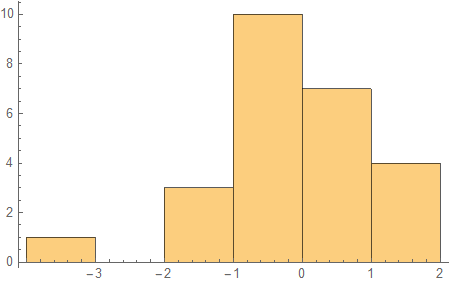
\includegraphics[width=0.45\textwidth]{imagenes2/histograma.png}
                  \caption{Histograma.}
              \end{subfigure}
              \begin{subfigure}[b]{0.45\textwidth}
                  \centering
                  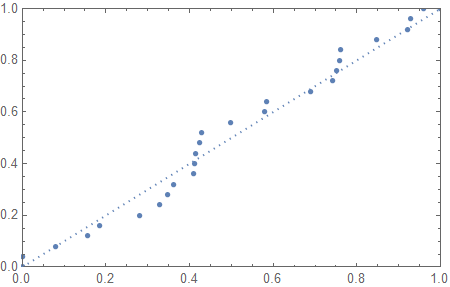
\includegraphics[width=0.45\textwidth]{imagenes2/probabilityplot.png}
                  \caption{Gráfico probabilístico normal.}
              \end{subfigure}
          \end{figure}
    \item \textbf{Gráfico de residuos frente a los valores predichos.}
          Sirve para comprobar si hay linealidad, homocedasticidad y datos atípicos.
          Se representan los residuos $t_i$ frente a los $\widehat{y_i}$.
          \begin{figure}[H]
              \centering
              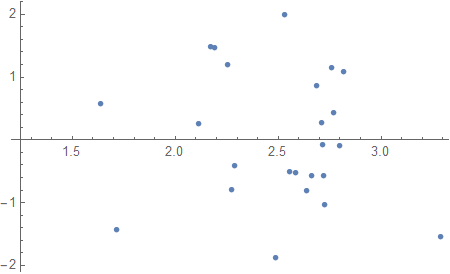
\includegraphics[width=0.5\textwidth]{imagenes2/resfrentepred.png}
          \end{figure}
    \item \textbf{Gráficos de residuos frente a variables explicativas.}
          Detectan si hay linealidad, homocedasticidad y datos atípicos en cada variable.
          Se hacen $k$ gráficos, cada uno representando los residuos $t_i$ frente a cada variable $X_{ji}$, para $j = 1, \dots, k$.
    \item \textbf{Gráficos parciales de residuos.}
          Miden la influencia de cada $X_i$ quitando todas las demás variables.
          Se hacen $k$ gráficos con el siguiente procedimiento para cada $X_i$ con $i = 1, \dots, k$:
          \begin{enumerate}
              \item Ajustamos el modelo con todas las variables explicativas salvo $X_i$.
              \item Calculamos los errores del ajuste anterior $t_j^{(i)}$ y los representamos frente a $X_i$.
          \end{enumerate}
    \item \textbf{Gráfico de residuos frente a variables omitidas.}
          Sirve para comprobar si una variable omitida $X_{k+1}$ debería ser tenida en cuenta en el modelo.
          Se representan los residuos frente a $X_{k+1}$.
          Una estructura lineal en esta gráfica indica que hay que tener en cuenta esta variable.
\end{enumerate}

\subsection{Observaciones atípicas e influyentes}

La observación $i$-ésima es atípica a nivel de significación $\alpha$ si $|t_i| > t_{n-k-2, 1-\frac{\alpha}{2}}$.

Una observación es influyente si se da alguno de estos casos:
\begin{itemize}
    \item Modifica el vector $\widehat{\vec{\beta}}$ de parámetros estimado.
    \item Modifica el vector $\widehat{\vec{y}}$ de predicciones.
    \item Hace que la observación del punto sea muy buena cuando este se incluye en el modelo y mala cuando se excluye.
\end{itemize}
En general son puntos palanca.

Definimos la distancia de Cook de la observación $i$-ésima como:
\begin{align*}
    \boxed{
        D(i) =  \frac{(\widehat{\vec{\beta}}-\widehat{\vec{\beta}}_{(i)})'X'X(\widehat{\vec{\beta}}-\widehat{\vec{\beta}}_{(i)})}{(k+1)s_R^2}
    }
\end{align*}
donde $\widehat{\vec{\beta}}_{(i)}$ es el vector de parámetros estimado sin la observación $i$-ésima.

\begin{obs}
    Recordamos que:
    \begin{align*}
        \begin{cases}
            \dfrac{(\widehat{\vec{\beta}}-\vec{\beta})'X'X(\widehat{\vec{\beta}}-\vec{\beta})}{\sigma^2} \sim \chi^2_{k+1} \\
            \dfrac{(n-k-1)s_R^2}{\sigma^2} = \dfrac{\sum e_i^2}{\sigma^2} \sim \chi^2_{n-k-1}
        \end{cases}
    \end{align*}
    Entonces:
    \begin{align*}
        \frac{\dfrac{(\widehat{\vec{\beta}}-\vec{\beta})'X'X(\widehat{\vec{\beta}}-\vec{\beta})}{\sigma^2} / (k+1)}{\dfrac{(n-k-1)s_R^2}{\sigma^2} / (n-k-1)} = \dfrac{(\widehat{\vec{\beta}}-\vec{\beta})'X'X(\widehat{\vec{\beta}}-\vec{\beta})}{(k+1)s_R^2} \sim F_{k+1, n-k-1}
    \end{align*}
\end{obs}
Usando esta distancia, podemos determinar que la observación $i$-ésima es influyente a nivel de significación $\alpha$ si:
\begin{align*}
    D(i) > F_{k+1, n-k-1, 1-\alpha}
\end{align*}

\begin{obs}
    Una distancia $D(i) > 1$ suele indicar que la observación es influyente.
\end{obs}

\section{Selección de modelos}
Distinguimos dos tipos de medidas para la bondad del modelo:
\begin{enumerate}
    \item Criterios basados en la bondas de ajuste:
          \begin{itemize}
              \item \textbf{Coeficiente de determinación.}
                    No sirve para comparar modelos en general, porque aquel que tenga más variables explicativas tiene un mayor $R^2$, incluso si no son significativas.
              \item \textbf{Coeficiente de determinación ajustado.}
                    Es mejor modelo el que tenga mayor $\overline{R}^2$.
              \item \textbf{Varianza residual.}
                    Es mejor modelo el que tenga menor $s_R^2$.
                    Es equivalente al anterior criterio por la relación que hay entre $\overline{R}^2$ y $s_R^2$.
          \end{itemize}
    \item Criterios basados en buscar buenas predicciones:
          \begin{itemize}
              \item \textbf{AIC (Akaike Information Criterion).}
                    Es mejor modelo el que tenga menor AIC.
              \item \textbf{BIC (Bayesian Information Criterion).}
                    Es mejor modelo el que tenga menor BIC.
          \end{itemize}
\end{enumerate}

Si dos modelos tienen una bondad similar, siempre es preferible el más simple.

\section{Regresión con variables cualitativas}
Supongamos que tenemos dos poblaciones demográficas $A$ y $B$ y tenemos unas variables aleatorias $X_1,\ldots,X_k$. Sean $x_{1i},\ldots,x_{ki}$ datos sobre dichas variables aleatorias que sabemos a que población corresponden. Podemos tener los siguientes modelos:
\begin{enumerate}
    \item Mezclar todos los datos y hacer una regresión lineal sobre ellos, es decir, consideramos el siguiente modelo
          \begin{align*}
              y_i = \beta_0 + \beta_1 x_{1i} +  \ldots + \beta_k x_{ki} + u_i,
          \end{align*}
          y lo estimamos de la siguiente forma,
          \begin{align*}
              \widehat{y}_i = \widehat{E(y_1 | x_{1i},\ldots,x_{ki})} = \widehat{\beta}_0 + \widehat{\beta}_1 x_{1i} + \ldots + \widehat{\beta}_k x_{ki}.
          \end{align*}
          Lo bueno de este modelo es que usamos todos los datos, pero estamos considerando que ambas poblaciones son homogéneas.
    \item Ajustar cada población por serparado, es decir, hacer una regresión lineal para la población $A$ y otra regresión lineal para la población $B$. Lo bueno de este modelo es que podemos hacer buenas estimaciones de ambas poblaciones de manera independiente, pero en cada modelo usamos menos datos.
    \item Introducir una nueva variable, $X_{k+1}$ (variable Dummy) tal que
          \begin{align*}
              x_{k+1,i} =  \begin{cases}
                               1, \text{ si el dato $i$-ésimo pertenece a la población $A$} \\
                               0, \text{ si el dato $i$-ésimo pertenece a la población $B$}
                           \end{cases} .
          \end{align*}
          Ahora, nuestros datos serían de la forma $(x_{1i}, x_{2i},\ldots, x_{ki}, \text{1 ó 0},y_i)$. Así, consideramos el modelo
          \begin{align*}
              \widehat{y}_i = \widehat{\beta}_0 + \widehat{\beta}_1 x_{1i} + \ldots + \widehat{\beta}_k x_{ki} + \widehat{\beta}_{k+1}x_{k+1,i}
          \end{align*}
          \begin{itemize}
              \item Para obtener la regresión para la población $A$ basta tomar $x_{k+1,i} = 1$,
                    \begin{align*}
                        \widehat{y}_i = \widehat{\beta}_0 + \widehat{\beta}_1 x_{1i} + \ldots + \widehat{\beta}_k x_{ki} + \widehat{\beta}_{k+1}
                    \end{align*}
              \item Para obtener la regresión para la población $B$ basta tomar $x_{k+1,i} = 0$,
                    \begin{align*}
                        \widehat{y}_i = \widehat{\beta}_0 + \widehat{\beta}_1 x_{1i} + \ldots + \widehat{\beta}_k x_{ki}
                    \end{align*}
          \end{itemize}
          Para saber si ambas poblaciones son homogéneas, o equivalentemente, si la variable $X_{k+1}$ es significativa, podemos plantear el siguiente contraste:
          \begin{align*}
              \begin{cases}
                  H_0 : \beta_{k+1} = 0 \\
                  H_1 : \beta_{k+1} \not = 0
              \end{cases}
          \end{align*}
\end{enumerate}
Los modelos que hemos visto se llaman modelos anidados, debido a que cada uno contiene todos los términos del modelo anterior. Este último es mejor que los anteriores pero supone que el incremento de $\widehat{y}$ es igual para cada población, lo que no es cierto en general. Veremos en ejemplos que podemos mejorarlo añadiendo interacciones.

\begin{ejemplo}
    Consideramos las variables $Y$ (peso en kg) y $X$ (altura en cm). Los datos $\{(x_i, y_i)\}$ provienen de dos poblaciones según el sexo: hombres y mujeres.

    El modelo conjunto sería:
    \begin{align*}
        \widehat{y} = \widehat{\beta}_0 + \widehat{\beta}_1x_1
    \end{align*}
    Como el sexo influye en el peso de una persona, añadimos una variable ficticia, $X_2$, para mejorar el modelo tal que
    \begin{align*}
        x_{2i} =  \begin{cases}
                      1, \text{ si el dato $i$-ésimo es hombre} \\
                      0, \text{ si el dato $i$-ésimo es mujer}.
                  \end{cases}
    \end{align*}
    Codificamos los datos a la forma $(x_{1i}, x_{2i}, y_i)$ para tener en cuenta estas nuevas variables.
    De esta forma, obtenemos el modelo general:
    \begin{align*}
        \widehat{y} = \widehat{\beta}_0 + \widehat{\beta}_1x_1 + \widehat{\beta}_2x_2
    \end{align*}
    Al término $\widehat{\beta}_2x_2$ se le llama \textbf{efecto principal} del tipo de combustible.
    \begin{itemize}
        \item Para los hombres el modelo es:
              \begin{align*}
                  \widehat{y} = \widehat{\beta}_0 + \widehat{\beta}_1x_1 + \widehat{\beta}_2 = (\widehat{\beta}_0 + \widehat{\beta}_2) + \widehat{\beta}_1x_1
              \end{align*}
        \item Para las mujeres el modelo es:
              \begin{align*}
                  \widehat{y} = \widehat{\beta}_0 + \widehat{\beta}_1x_1
              \end{align*}
    \end{itemize}

    Podemos observar que ambas rectas tienen la misma pendiente, es decir, se supone que el incremento de los pesos es igual en cada población, lo que no es cierto en general.  Para mejorar el modelo, introducimos un nuevo término $\widehat{\beta}_3x_1x_2$ llamado \textbf{interacción} de altura y sexo. Así que este nuevo modelo queda de la forma:
    \begin{align*}
        \widehat{y} = \widehat{\beta}_0 + \widehat{\beta}_1x_1 + \widehat{\beta}_2x_2 + \widehat{\beta}_3x_1x_2
    \end{align*}
    \begin{itemize}
        \item Para los hombres el modelo es:
              \begin{align*}
                  \widehat{y} = \widehat{\beta}_0 + \widehat{\beta}_1x_1 + \widehat{\beta}_2 + \widehat{\beta}_3x_1 = (\widehat{\beta}_0 + \widehat{\beta}_2) + (\widehat{\beta}_1 + \widehat{\beta}_3)x_1
              \end{align*}
        \item Para las mujeres el modelo es:
              \begin{align*}
                  \widehat{y} = \widehat{\beta}_0 + \widehat{\beta}_1x_1
              \end{align*}
    \end{itemize}
    Observamos que ahora las rectas tienen distinta pendiente.

    Podemos realizar algunos contrastes de hipótesis para comprobar si este modelo es el correcto. Para determinar si el sexo tiene una influencia significativa en el peso, contrastamos:
    \begin{align*}
        \begin{cases}
            H_0: \beta_2 = \beta_3 = 0 \\
            H_1: \beta_2 \neq 0 \text{ o } \beta_3 \neq 0
        \end{cases}
    \end{align*}
    Para comprobar si el incremente en el peso medio es igual para hombres y mujeres, podemos realizar el contraste:
    \begin{align*}
        \begin{cases}
            H_0: \beta_3 = 0 \\
            H_1: \beta_3 \neq 0
        \end{cases}
    \end{align*}
\end{ejemplo}

\begin{ejemplo}
    Consideramos las variables $Y$ (rendimiento de un motor diésel) y $X$ (velocidad del motor).
    Existen tres tipos de combustible: petróleo, carbón y mezcla. Tenemos un conjunto de datos $\{(x_i, y_i)\}$ con los distintos tipos de combustible y queremos ajustar un modelo de regresión.

    El modelo conjunto sería:
    \begin{align*}
        \widehat{y} = \widehat{\beta}_0 + \widehat{\beta}_1x_1
    \end{align*}
    Como es de esperar que el tipo de combustible influya en el rendimiento del motor, añadimos dos variables ficticias, $X_2$ y $X_3$ tales que:
    \begin{align*}
        x_{2i} & =  \begin{cases}
                        1, \text{ si el dato $i$-ésimo usa petróleo} \\
                        0, \text{ si el dato $i$-ésimo no usa patróleo}.
                    \end{cases} \\
        x_{3i} & =  \begin{cases}
                        1, \text{ si el dato $i$-ésimo usa carbón} \\
                        0, \text{ si el dato $i$-ésimo no usa carbón}.
                    \end{cases}
    \end{align*}
    Codificamos los datos a la forma $(x_{1i}, x_{2i}, x_{3i}, y_i)$ para tener en cuenta estas nuevas variables. De esta forma, obtenemos el modelo general:
    \begin{align*}
        \widehat{y} = \widehat{\beta}_0 + \widehat{\beta}_1x_1 + \widehat{\beta}_2x_2 + \widehat{\beta}_3x_3
    \end{align*}
    Al término $\widehat{\beta}_2x_2 + \widehat{\beta}_3x_3$ se le llama \textbf{efecto principal} del tipo de combustible.
    \begin{itemize}
        \item Para el petróleo el modelo es:
              \begin{align*}
                  \widehat{y} = \widehat{\beta}_0 + \widehat{\beta}_1x_1 + \widehat{\beta}_2 = (\widehat{\beta}_0 + \widehat{\beta}_2) + \widehat{\beta}_1x_1
              \end{align*}
        \item Para el carbón el modelo es:
              \begin{align*}
                  \widehat{y} = \widehat{\beta}_0 + \widehat{\beta}_1x_1 + \widehat{\beta}_3 = (\widehat{\beta}_0 + \widehat{\beta}_3) + \widehat{\beta}_1x_1
              \end{align*}
        \item Para la mezcla el modelo es:
              \begin{align*}
                  \widehat{y} = \widehat{\beta}_0 + \widehat{\beta}_1x_1
              \end{align*}
    \end{itemize}
    De nuevo, podemos observar que las tres rectas tienen la misma pendiente, es decir, se supone que el incremento del rendimiento del motor es igual para cada tipo de combustible, lo que no es cierto en general. Para corregirlo introducimos la \textbf{interacción} entre velocidad y tipo de combustible $\widehat{\beta}_4x_1x_2 + \widehat{\beta}_5x_1x_3$. Así, el nuevo modelo queda de la forma:
    \begin{align*}
        \widehat{y} = \widehat{\beta}_0 + \widehat{\beta}_1x_1 + \widehat{\beta}_2x_2 + \widehat{\beta}_3x_3 + \widehat{\beta}_4x_1x_2 + \widehat{\beta}_5x_1x_3
    \end{align*}
    \begin{itemize}
        \item Para el petróleo el modelo es:
              \begin{align*}
                  \widehat{y} = \widehat{\beta}_0 + \widehat{\beta}_1x_1 + \widehat{\beta}_2 + \widehat{\beta}_4x_1 = (\widehat{\beta}_0 + \widehat{\beta}_2) + (\widehat{\beta}_1 + \widehat{\beta}_4)x_1
              \end{align*}
        \item Para el carbón el modelo es:
              \begin{align*}
                  \widehat{y} = \widehat{\beta}_0 + \widehat{\beta}_1x_1 + \widehat{\beta}_3 + \widehat{\beta}_5x_1 = (\widehat{\beta}_0 + \widehat{\beta}_3) + (\widehat{\beta}_1 + \widehat{\beta}_5)x_1
              \end{align*}
        \item Para la mezcla el modelo es:
              \begin{align*}
                  \widehat{y} = \widehat{\beta}_0 + \widehat{\beta}_1x_1
              \end{align*}
    \end{itemize}
    Ahora las rectas tienen distinta pendiente, como queríamos.

    También podemos realizar algunos contrastes de hipótesis para comprobar si este modelo es el correcto. Para determinar si el rendimiento medio del motor depende del tipo de combustible, contrastamos:
    \begin{align*}
        \begin{cases}
            H_0: \beta_2 = \beta_3 = \beta_4 = \beta_5 = 0 \\
            H_1: \beta_2 \neq 0 \text{ o } \beta_3 \neq 0 \text{ o } \beta_4 \neq 0 \text{ o } \beta_5 \neq 0
        \end{cases}
    \end{align*}
    Para comprobar si hay dependencia entre velocidad y tipo de combustible, podemos realizar el contraste:
    \begin{align*}
        \begin{cases}
            H_0: \beta_4 = \beta_5 = 0 \\
            H_1: \beta_4 \neq 0 \text{ o } \beta_5 \neq 0
        \end{cases}
    \end{align*}
    Supongamos ahora que creemos que la relación entre el rendimiento medio de un motor diésel y la veloicidad es cuadrática. Entonces el modelo conjunto sería:
    \begin{align*}
        \widehat{y} = \widehat{\beta}_0 + \widehat{\beta}_1x_1 + \widehat{\beta}_2x_1^2
    \end{align*}
    Añadimos el efecto principal del tipo de combustible con las variables ficticias $X_2$ y $X_3$:
    \begin{align*}
        \widehat{y} = \widehat{\beta}_0 + \widehat{\beta}_1x_1 + \widehat{\beta}_2x_1^2 + \widehat{\beta}_3x_2 + \widehat{\beta}_4x_3
    \end{align*}
    \begin{itemize}
        \item Para el petróleo el modelo es:
              \begin{align*}
                  \widehat{y} = \widehat{\beta}_0 + \widehat{\beta}_1x_1 + \widehat{\beta}_2x_1^2 + \widehat{\beta}_3 = (\widehat{\beta}_0 + \widehat{\beta}_3) + \widehat{\beta}_1x_1 + \widehat{\beta}_2x_1^2
              \end{align*}
        \item Para el carbón el modelo es:
              \begin{align*}
                  \widehat{y} = \widehat{\beta}_0 + \widehat{\beta}_1x_1 + \widehat{\beta}_2x_1^2 + \widehat{\beta}_4 = (\widehat{\beta}_0 + \widehat{\beta}_4) + \widehat{\beta}_1x_1 + \widehat{\beta}_2x_1^2
              \end{align*}
        \item Para la mezcla el modelo es:
              \begin{align*}
                  \widehat{y} = \widehat{\beta}_0 + \widehat{\beta}_1x_1 + \widehat{\beta}_2x_1^2
              \end{align*}
    \end{itemize}
    Añadimos ahora la interacción entre la velocidad del motor y el tipo de combustible:
    \begin{align*}
        \widehat{y} = \widehat{\beta}_0 + \widehat{\beta}_1x_1 + \widehat{\beta}_2x_1^2 + \widehat{\beta}_3x_2 + \widehat{\beta}_4x_3 + \widehat{\beta}_5x_1x_2 + \widehat{\beta}_6x_1x_3 + \widehat{\beta}_7x_1^2x_2 + \widehat{\beta}_8x_1^2x_3
    \end{align*}
    \begin{itemize}
        \item Para el petróleo el modelo es:
              \begin{align*}
                  \widehat{y} = \widehat{\beta}_0 + \widehat{\beta}_1x_1 + \widehat{\beta}_2x_1^2 + \widehat{\beta}_3 + \widehat{\beta}_5x_1 + \widehat{\beta}_7x_1^2 = (\widehat{\beta}_0 + \widehat{\beta}_3) + (\widehat{\beta}_1 + \widehat{\beta}_5)x_1 + (\widehat{\beta}_2 + \widehat{\beta}_7)x_1^2
              \end{align*}
        \item Para el carbón el modelo es:
              \begin{align*}
                  \widehat{y} = \widehat{\beta}_0 + \widehat{\beta}_1x_1 + \widehat{\beta}_2x_1^2 + \widehat{\beta}_4 + \widehat{\beta}_6x_1 + \widehat{\beta}_8x_1^2 = (\widehat{\beta}_0 + \widehat{\beta}_4) + (\widehat{\beta}_1 + \widehat{\beta}_6)x_1 + (\widehat{\beta}_2 + \widehat{\beta}_8)x_1^2
              \end{align*}
        \item Para la mezcla el modelo es:
              \begin{align*}
                  \widehat{y} = \widehat{\beta}_0 + \widehat{\beta}_1x_1 + \widehat{\beta}_2x_1^2
              \end{align*}
    \end{itemize}
    Para determinar si el modelo medio de un motor varía según el tipo de combustible, contrastamos:
    \begin{align*}
        \begin{cases}
            H_0: \beta_i = 0, \quad \forall i \in \{3,\ldots,8\} \\
            H_1 : \exists i \in \{3,\ldots,8\} : \beta_i \not = 0
        \end{cases}
    \end{align*}
    Para comprobar si un modelo de segundo orden es mejor a uno de primer orden, realizamos el contraste:
    \begin{align*}
        \begin{cases}
            H_0: \beta_2 = \beta_7 = \beta_8 = 0 \\
            H_1: \exists i \in \{2,7,8\} : \beta_i \not = 0
        \end{cases}
    \end{align*}
\end{ejemplo}